% to do
% 1. show that the covariance scale as the amplitude
% 2. Try with Gaussian covariance

\documentclass[fleqn, usenatbib]{mnras}
\usepackage{style}                                          % the settings are all here 
\newcommand{\Ng}{N_\mathrm{g}}
\newcommand{\Bsmooth}{B_\mathrm{smooth}}
\newcommand{\Bbao}{B_\mathrm{BAO}}

\title[Constraining BAO with DESI]{Constraining BAO parameter with Bispectrum clustering of DESI Tracers}
% If you need two or more lines of authors, add an extra line using \newauthor
\author[Doe et al.]{Stephen Hawking$^{1,2}$, Albert Einstein$^{3}$, Bernie Sanders$^{4}$, \newauthor
Next Author$^{4}$
\\~\\
% List of institutions
$^{1}$Department of Physics, Kansas State University, 116 Cardwell Hall, Manhattan, KS 66506, USA\\
$^{2}$Department of Physics and Astronomy, Ohio University, Athens, OH 45701, USA\\
$^{3}$Center for Cosmology and AstroParticle Physics, The Ohio State University, 191 West Woodruff Avenue, Columbus, OH 43210, USA\\
$^{4}$IRFU, CEA, Universite Paris-Saclay, F-91191 Gif-sur-Yvette, France\\
}

% Don't touch these lines
\begin{document}
\label{firstpage}
\pagerange{\pageref{firstpage}--\pageref{lastpage}}
\maketitle


\begin{abstract}
We use simulations with and without BAO signal to assess the possibility of extracting more information from higher order statistics. We measure the BAO constraints from the power spectrum and the bispectrum of DESI-like LRG tracers. We show that the BAO signal in the bispectrum has a potential of significantly improving the distance constraints by X\% compared to the power spectrum alone analysis. The improvement seems to be stable when we marginalize over possible theoretical systematics. We validate our results on simulations with and without BAO for a range of redshifts. We measure isotropic BAO from the AbacusSummit simulations that are designed to replicate the DESI BGS, LRG, ELG, and QSO samples. We find that, in the absence of additional systematic effects we are able to constrain the distance scale with the precision of xxx per cent, xxx per cent, and xxx percent respectively for the BGS, LRG, and ELG samples. Whereas, the forecasted BAO constraints for the power spectrum only are xxx, xxx, and xxx percent respectively.
\end{abstract}


% Select between one and six entries from the list of approved keywords.
% Don't make up new ones.
\begin{keywords}
Awesome keywords: Perfect
\end{keywords}


%%%%%%%%%%%%%%%%% BODY OF PAPER 
\section{Introduction}
\label{sec:introduction}

DESI is a great experiment. We need higher order statistics to extract more information. Reconstruction techniques can improve the precision, but the amount of information is limited by cosmic variance. Possible ways to improve is to go higher order statistics. 

Cite Lado's paper that if bispectrum used as a standard ruler, a significant improvement is distance scale can be achieved. Much better than the standard reconstruction. Difficult to model the full bispectrum though. In this paper, we would like to do a standard ruler analysis of bispectrum BAO with different DESI-like tracers. 

We find a factor of X improvement, and what happens at different redshifts. Worse for QSO probably, because of high shotnoise and less bispectrum clustering at higher redshifts. 


Sec 2. Glam Section
Plot Glam with and without BAO measurements.
Describe Molino's covariance and put some justification. 1 Gpc cub.
Reference Jayashree's paper that the template works well for a range of redshifts. make a plot for sigma alpha vs kmax, with and without nuisance parameters.
Use CAMB to get the bao constraints for reconstructed power spectrum with GLAM parameters.
Sec 3. BAO is DESI samples. Analyse Abacus mocks with template from Jayashree. Renormalize Molino's covariance by the ratio of spectra to get covariance for Abacus. Maybe use Glam and Molino to show that spectra ratio scales proportional to dispersion ratio.

Sec 4. BAO detection level. How well we can fit BAO with a smooth function. Mean Glam' with and without BAO as model 1 and 2, and mean Glam with BAO as data. Chi2 vs alpha.



\begin{equation}
\log \mathcal{L} = \Delta r^{\dagger} C^{-1} \Delta r,
\end{equation}
where $\Delta r = r(\textbf{k}) - r(\alpha \textbf{k})$ with $r$ being defined as the ratio of





\section{Simulations}
\label{sec:simulations}

To assess the nature of the BAO signal in the DESI bispectrum we use \texttt{FirstGen} simulations. These simulations are based on \texttt{AbacusSummit} N-body simulations. The halos in the \texttt{AbacusSummit} have been populated with galaxies using the \textcolor{red}{we will describe how the FirstGens were produced here}. These HOD parameters were derived by fitting the projected small-scale clustering of the DESI Early Data Release sample. 

We use \texttt{Molino} simulations to assist in constructing covariance matrices. \texttt{Molino} simulations are based on the \texttt{Quijote} N-body simulation suit. They were constructed by \textcolor{red}{Same thing here}.

We use the \texttt{GLAM} simulations for constructing some of our BAO fitting templates. \textcolor{red}{we will describe the volume the number, etc}. Each instance of the \texttt{GLAM} simulations was run with a paired simulation with no input BAO signal. 

Molino (15,000 Mocks): 
$\Omega_{M}=0.32$, $\sigma_{8}=0.834$, Volume $\sim 1 {\rm Gpc}/h^{3}$ 
Galaxy catalogs from the Quijote N-body simulations (Villaescusa-Navarro et al.2020) with the standard Halo Occupation Distribution model from Zheng et al. (2007). HOD parameters are based on high luminosity SDSS samples. More at changhoonhahn.github.io/molino

And two other series of mocks provided by our DESI collaborators:
GLAM (1,000 Mocks)

Abacus (25 mocks)


Fig. \ref{fig:data} shows the mean bispectrum (left) and the mean power spectrum (right) for the GLAM and ABACUS simulations, relative to the spectra without the BAO signal, which is simulation-based for the GLAM realizations and theory-based for the ABACUS.

\begin{figure*}
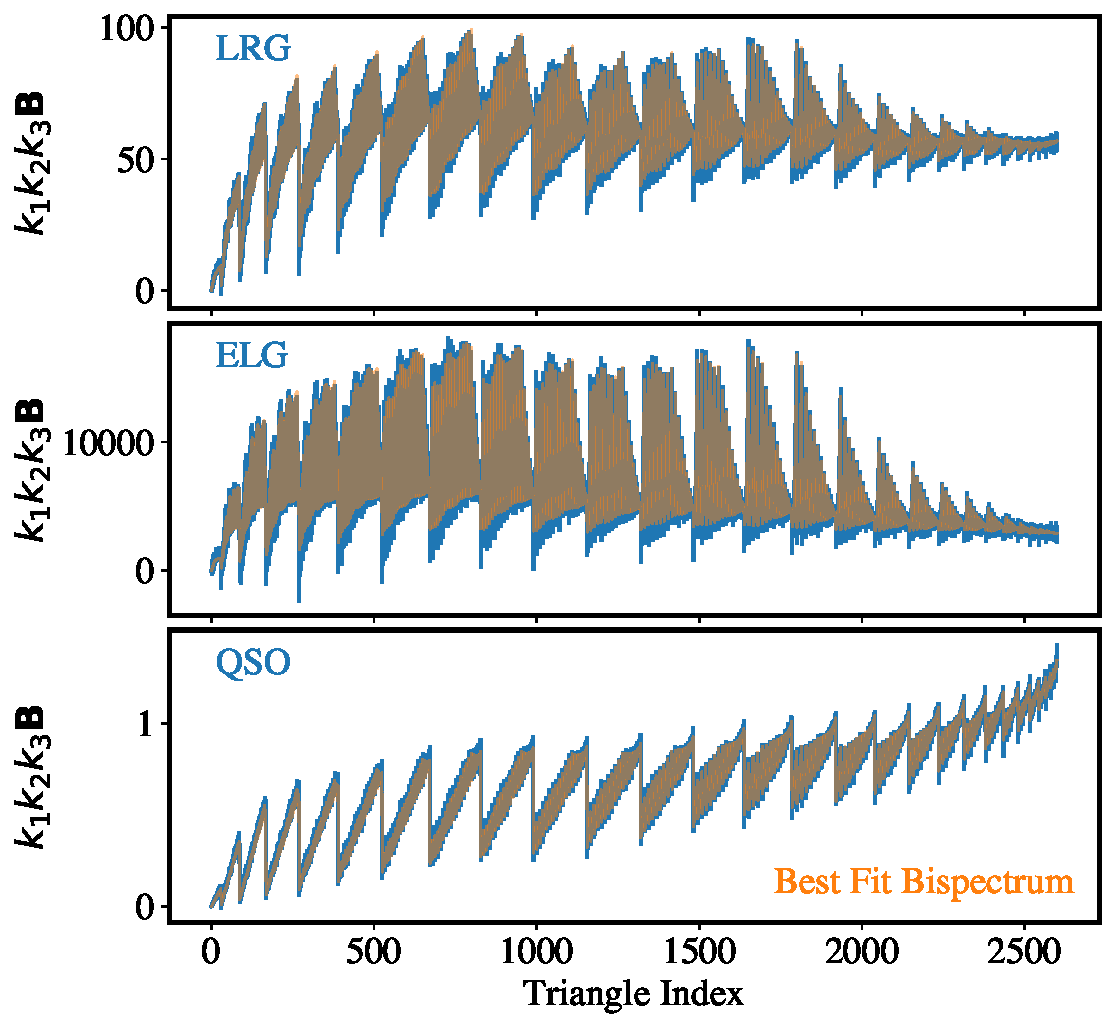
\includegraphics[width=\textwidth]{figures/spectra.pdf}
\caption{Spectra of ABACUS, GLAM, and MOLINO simulations. Top: Mean bispectrum and power spectrum of simulations relative to smooth spectrum either from the mocks (GLAM) or fitting formula (ABACUS). Bottom: Normalized dispersion of bispectrum and power spectrum.}\label{fig:data}
\end{figure*}


We estimate the reduced covariance matrix from a suite of 15000 simulations (MOLINO) and scale it by the variance of power spectrum or bispectrum for the GLAM or ABACUS realizations.
\section{DESI Measurements}\label{sec:measurements}

We measure bispectrum using standard techniques described in \cite{}. We start by dividing the cubic volume of simulations into $\Ng \times \Ng\times\Ng$ sized three-dimensional grid, where $\Ng = 1024$.

\textcolor{red}{LS: I will put a description of the entire algorithm here later. Also here we should describe the triangular index and the kinds of reductions that we do.}

We separate the bispectrum into smooth and BAOonly parts similar to how it's done for the power spectrum. We find functions $\Bsmooth$, and $\Bbao$ such that
\begin{equation}
    B = \Bsmooth\Bbao.
\end{equation}
$\Bsmooth$ models the bispectrum with the BAO signature removed. Even though its meaning is clear, it can not be rigorously defined from the first principles, which makes the separation into the smooth and BAO components part of the modeling. For a useful extracting we want the $\Bbao$ component to be oscillating around 1 and decay at higher wavenumbers. By constraining ourselves to the BAO-only analysis we are hoping that while our models for the $\Bsmooth$ may fail, the same models for the $\Bbao$ component will remain accurate.


Points on figure~\ref{fig:spectra} show the bispectrum of \textit{FirstGen} mocks as a function of the triangular index. The error bars are estimated from the variance of the 25 \textit{FirstGen} mocks for each tracer. The lines are the best-fit models from the leading order perturbation theory model \mr{(see Behera et al in prep)}, where the cosmological parameters have been fixed to the true values of the mocks and bias parameters were allowed to freely vary. The ELG tracers show the strongest clustering signal while the QSO sample show the weakest clustering signal which is dominated by shotnoise on small scales (large triangle indices). 

Figure~\ref{fig:spectra_ratio} shows the same measurements but divided by the smooth part of the bispectrum. \textcolor{red}{We will describe here what we see. Does the extraction always work well? high k problems?}. Figres~\ref{fig:spectra_ratio_reduced} show the reduced measurements for the $\Bbao$.

Figure~\ref{fig:powerspectra_ratio} shows the BAO-only power spectrum from the same simulations. 

Figure~\ref{fig:correlation} shows the bin-by-bin correlation of the bispectrum and power spectrum measurements.





\begin{figure}
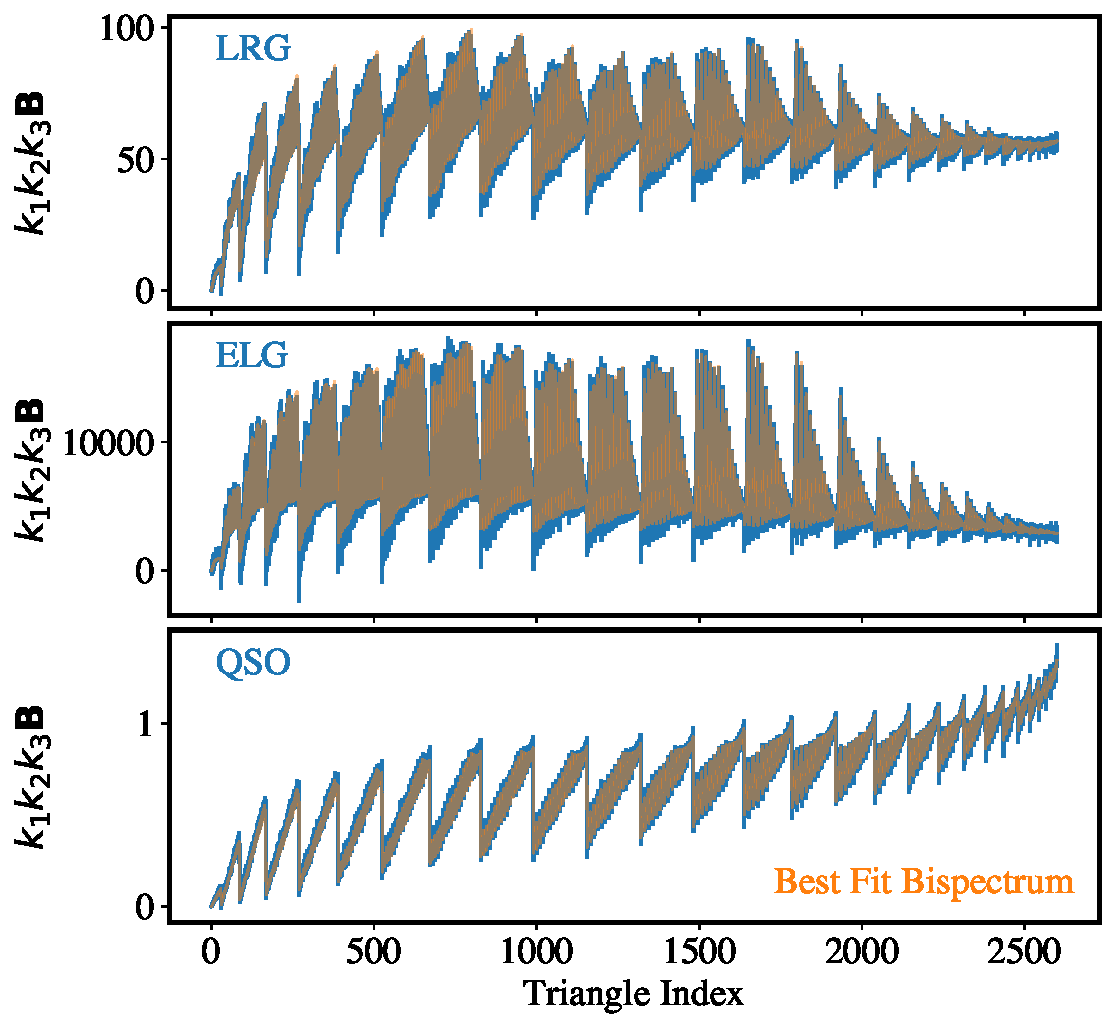
\includegraphics[width=0.45\textwidth]{figures/spectra.pdf}
\caption{Mean bispectrum of the Abacus LRG, ELG, and QSO simulations, repsectively, from top to bottom.}\label{fig:spectra}
\end{figure}

\begin{figure}
    \centering
    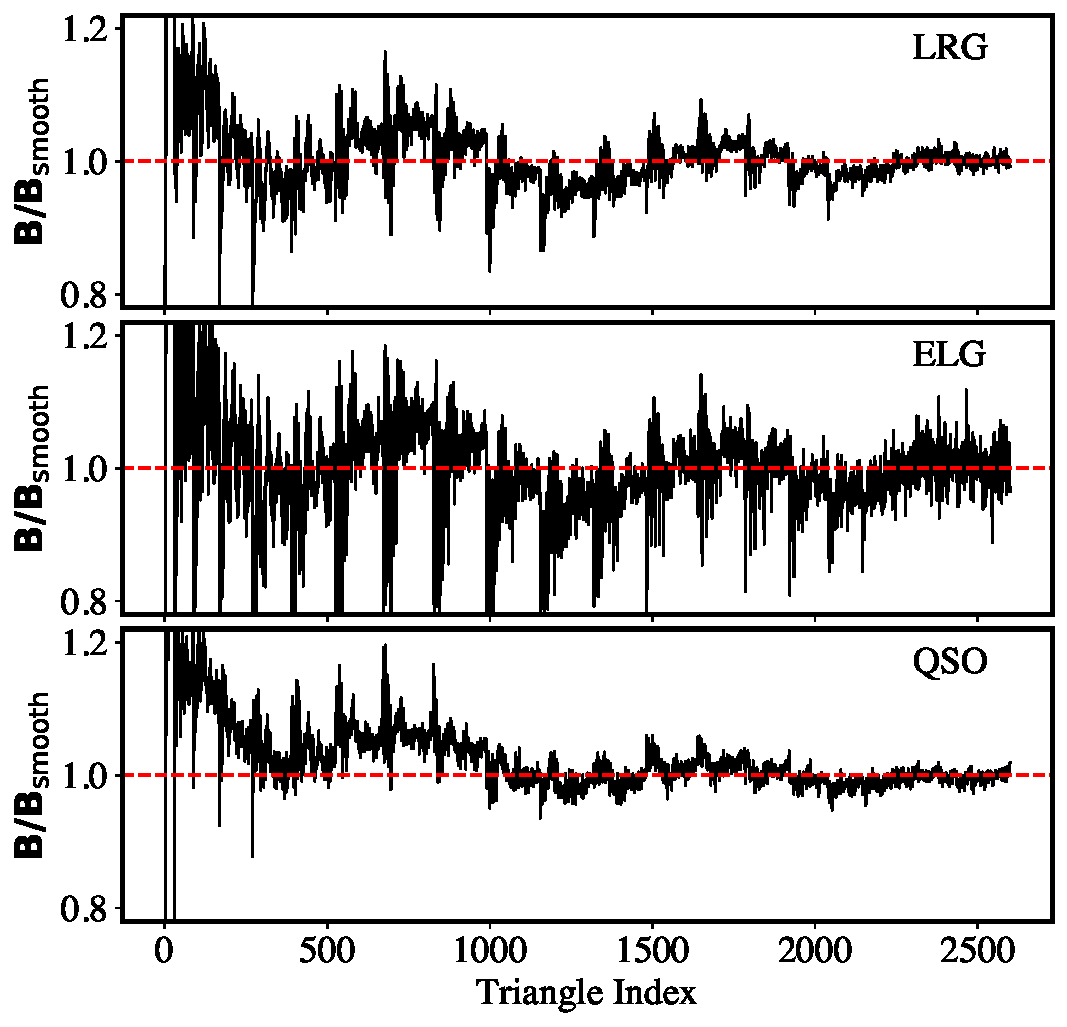
\includegraphics[width=0.45\textwidth]{figures/spectra_ratio.pdf}
    \caption{Same as Figure \ref{fig:spectra} for the ratio of bispectrum to smooth bispectrum.}
    \label{fig:spectra_ratio}
\end{figure}


\begin{figure}
    \centering
    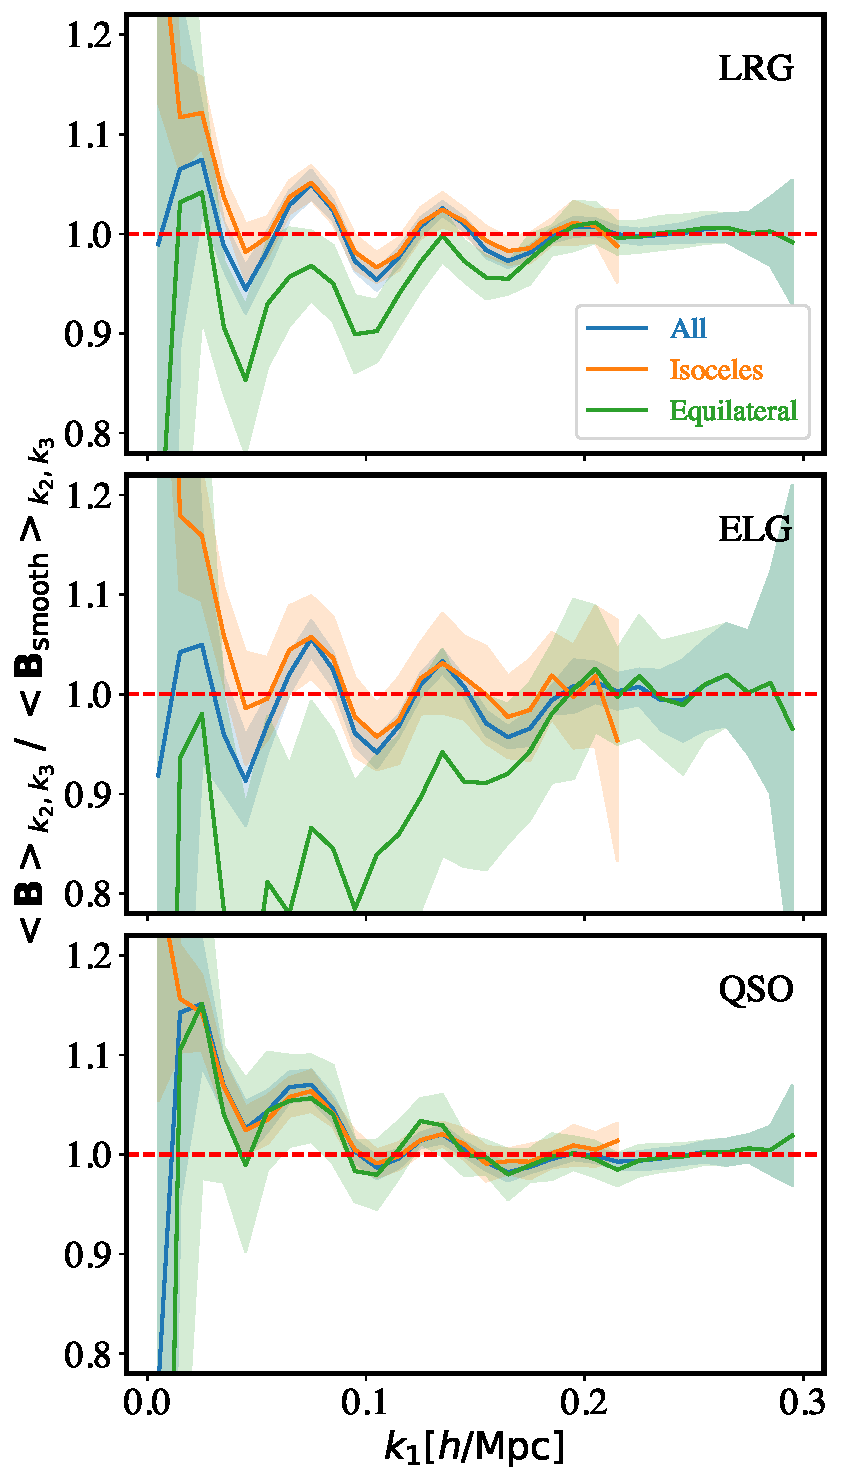
\includegraphics[width=0.45\textwidth]{figures/spectra_ratio_reduced.pdf}
    \caption{Same as Figure \ref{fig:spectra_ratio} for the reduced bispectrum.}
    \label{fig:spectra_ratio_reduced}
\end{figure}


\begin{figure}
    \centering
    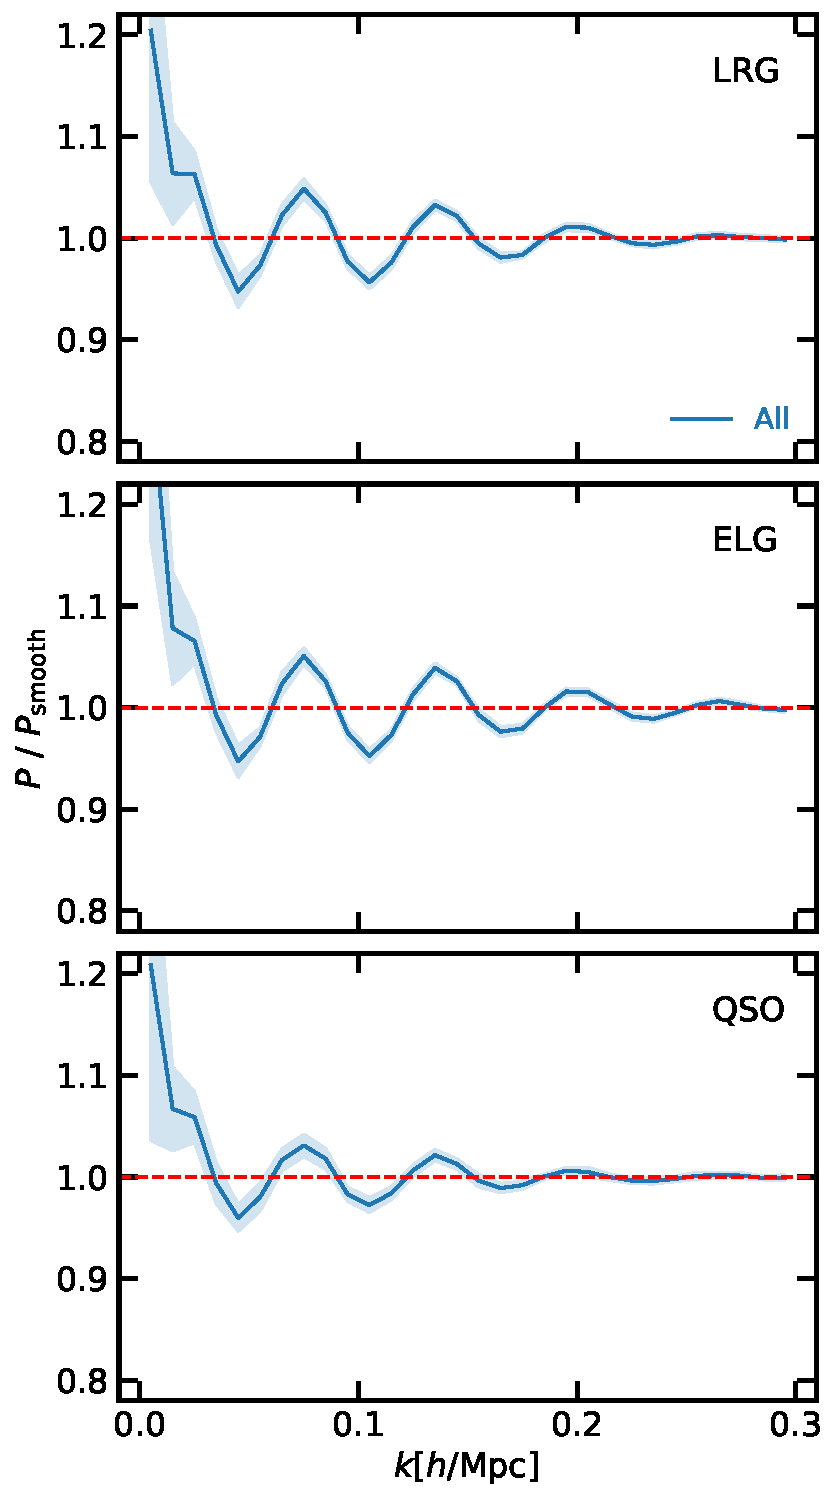
\includegraphics[width=0.45\textwidth]{figures/powerspectra_ratio.pdf}
    \caption{The ratio of the mean power spectrum to the mean smooth power spectrum.}
    \label{fig:powerspectra_ratio}
\end{figure}


\begin{figure*}
    \centering
    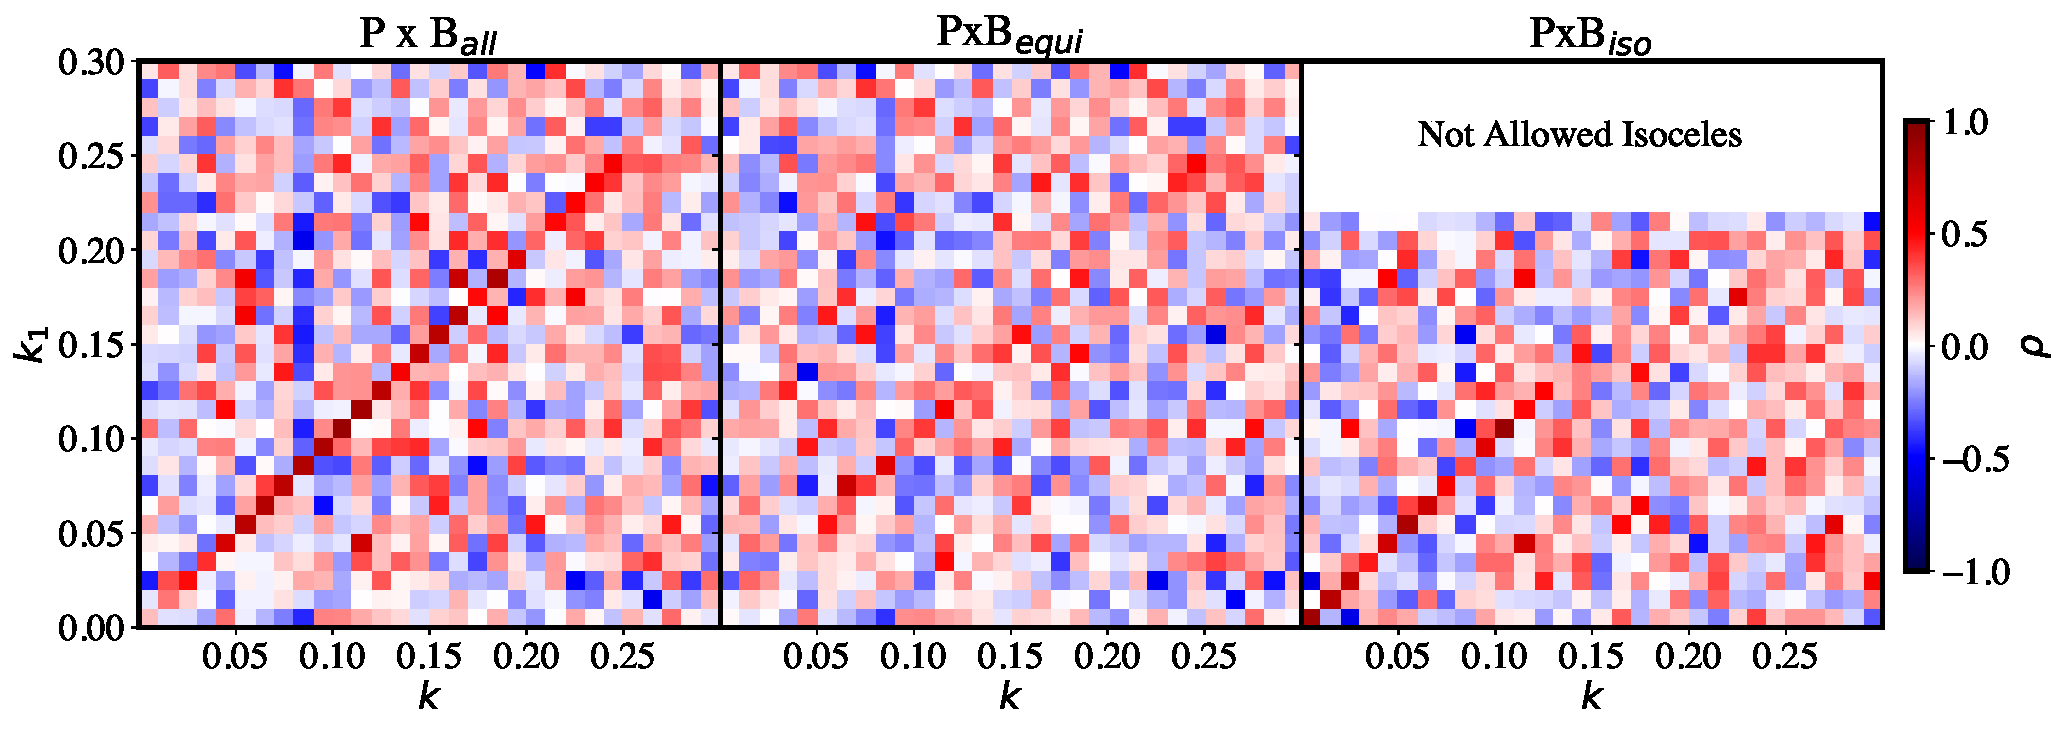
\includegraphics[width=\textwidth]{figures/corrmax_lrg.pdf}
    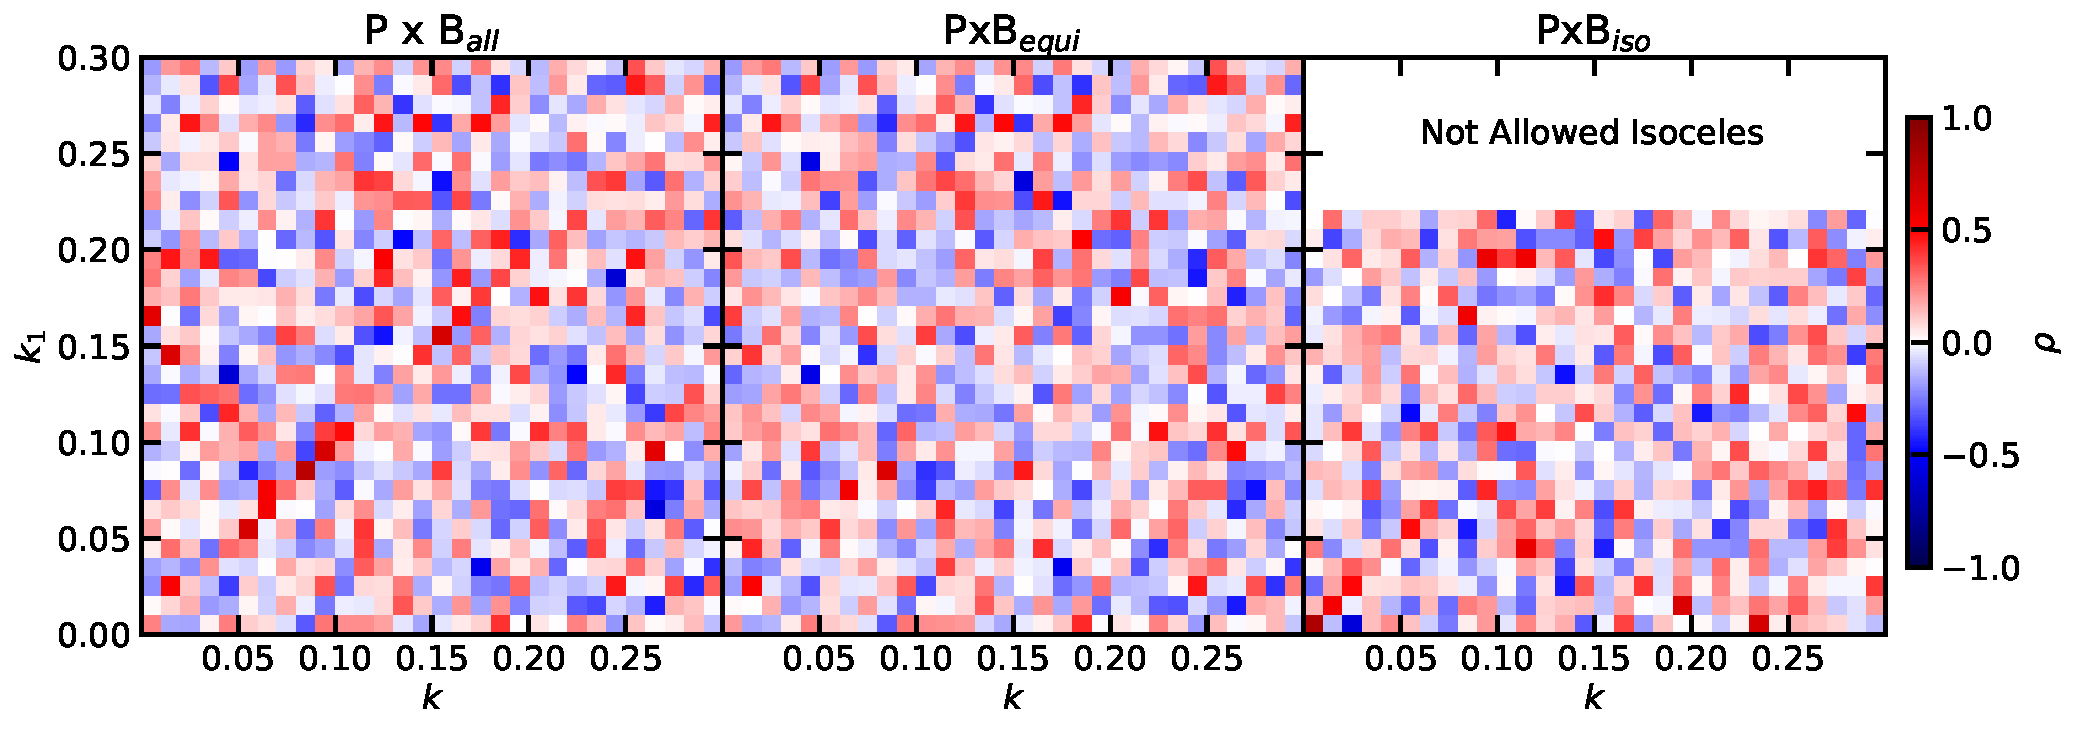
\includegraphics[width=\textwidth]{figures/corrmax_elg.pdf}
    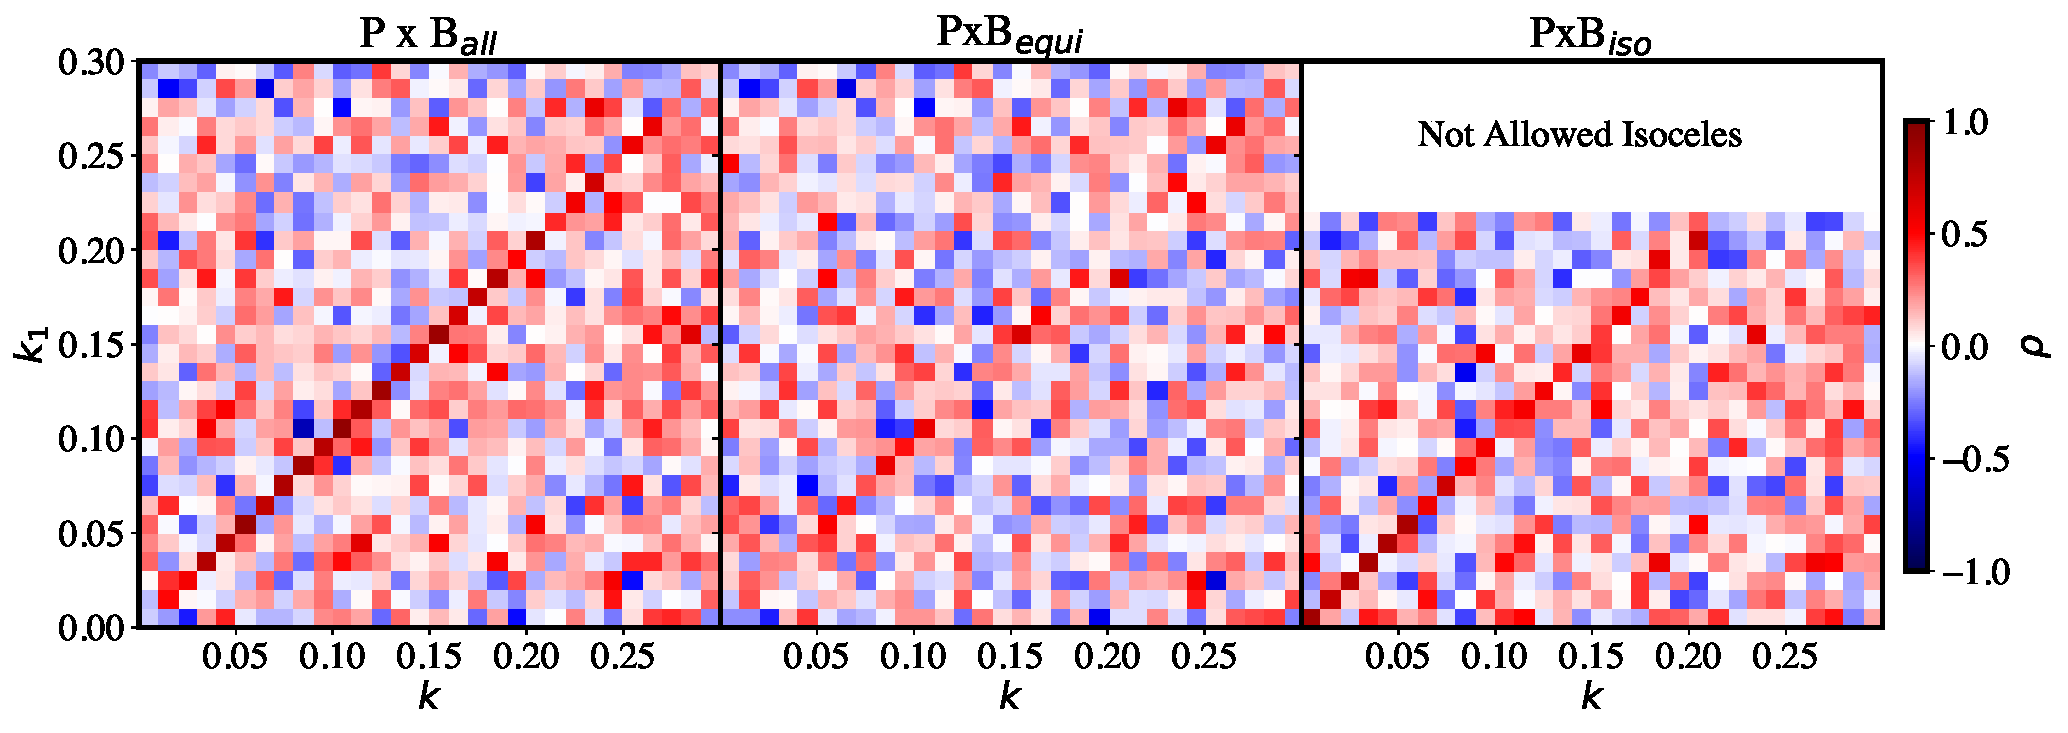
\includegraphics[width=\textwidth]{figures/corrmax_qso.pdf}
    \caption{The bin-by-bin correlation of the reduced bispectrum and power spectrum measurements for ABACUS LRG, ELG, and QSO samples. The left to right panel show different bispectrum configurations, respectively, all, equilateral, and isosceles.}
    \label{fig:correlation}
\end{figure*}


\begin{figure*}
    \centering
    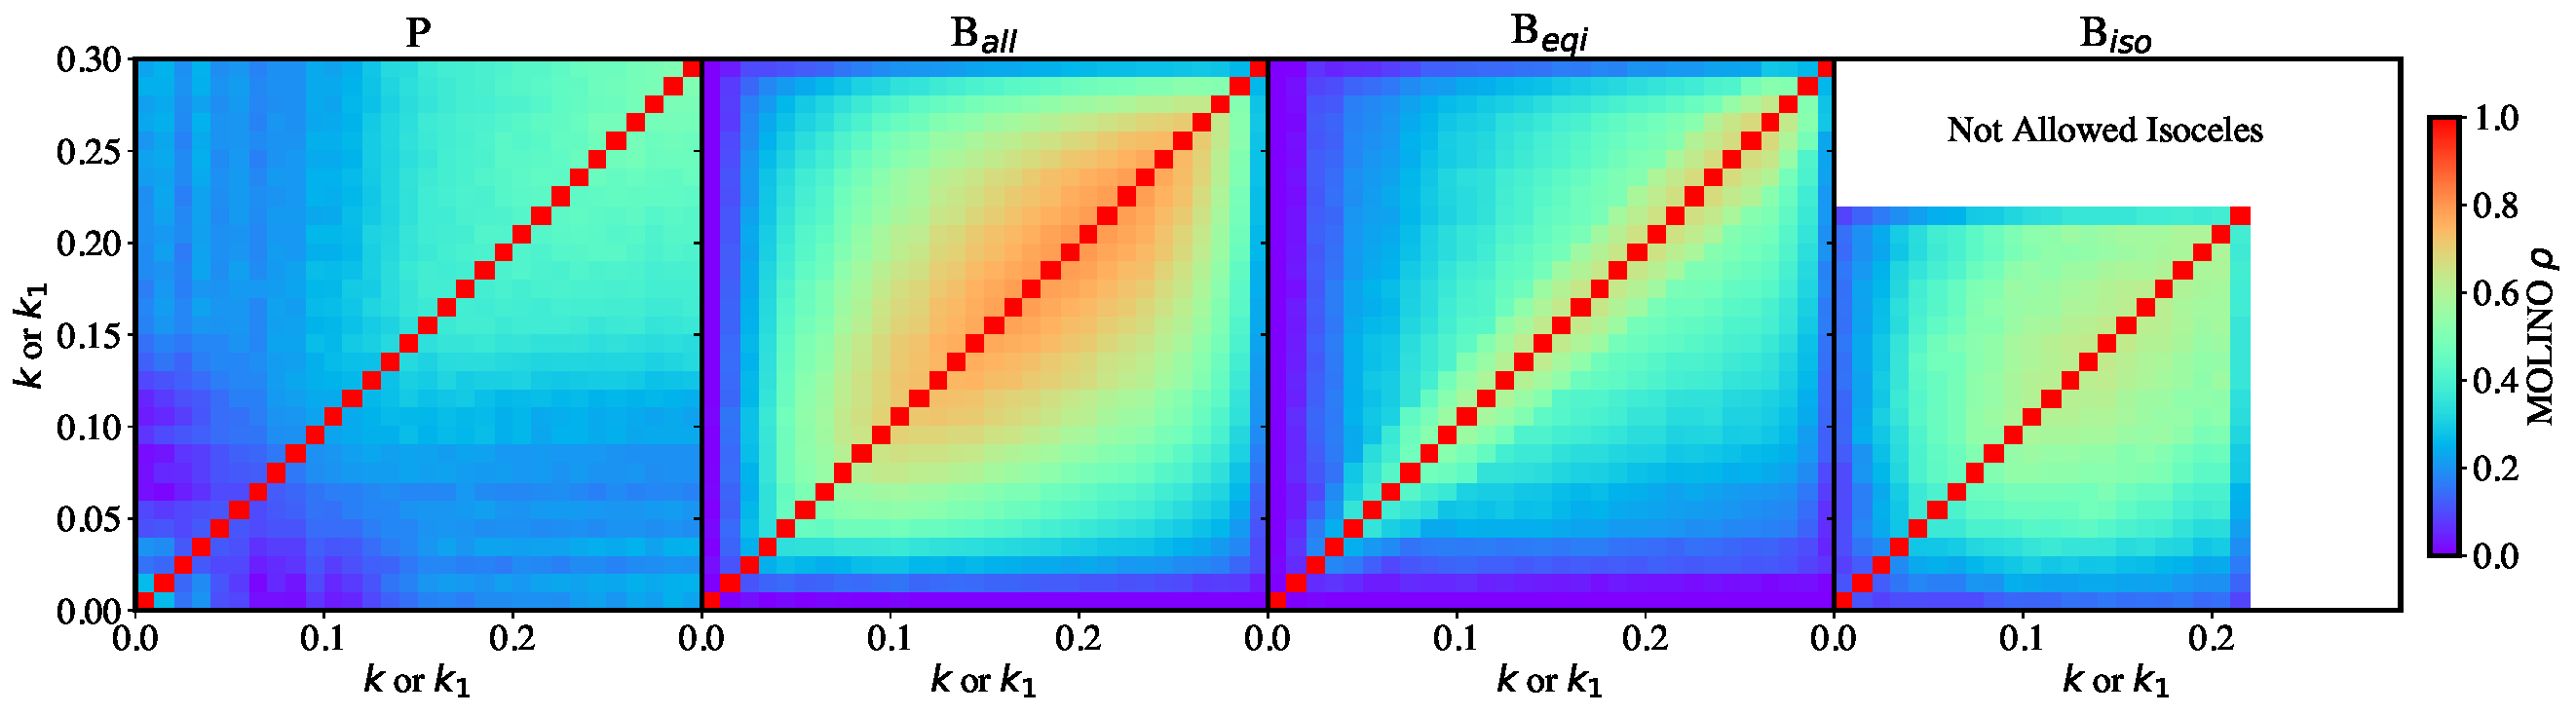
\includegraphics[width=\textwidth]{figures/corrmax_molino.pdf}
    \caption{Bin-by-bin auto-correlation of Molino power spectrum and reduced bispectrum.}
    \label{fig:correlation_molino}
\end{figure*}




\begin{figure*}
    \centering
    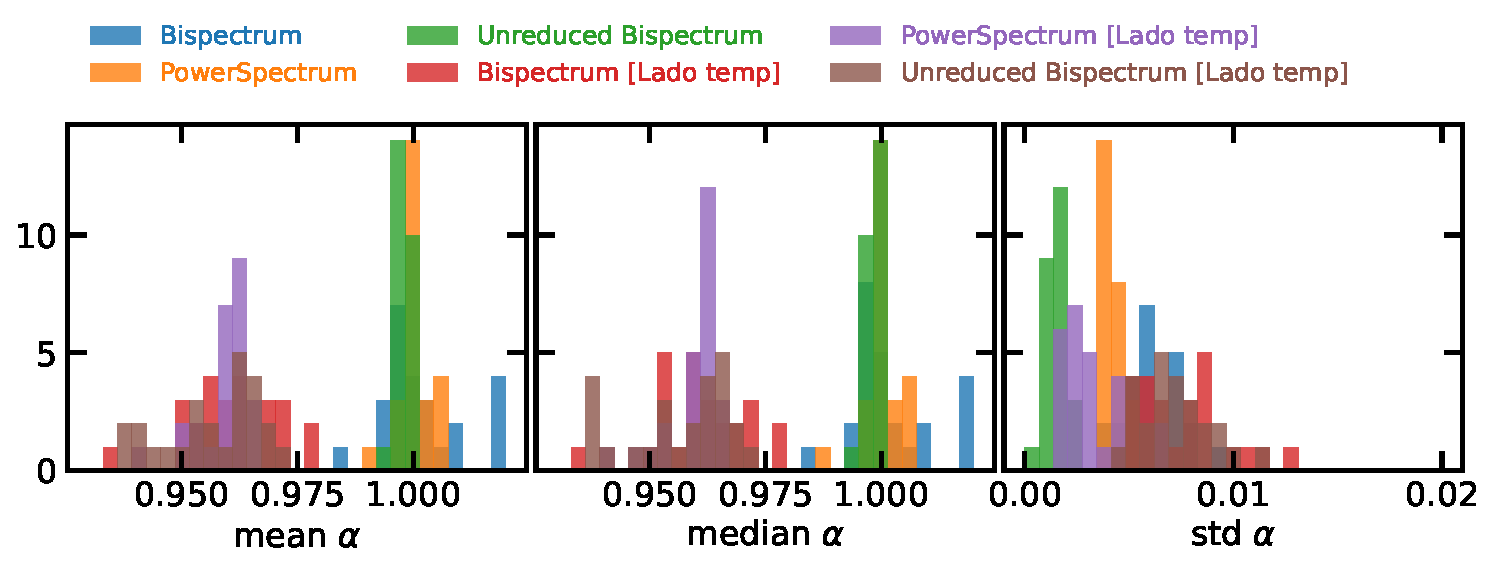
\includegraphics[width=\textwidth]{figures/constraints_LRGz0.pdf}
    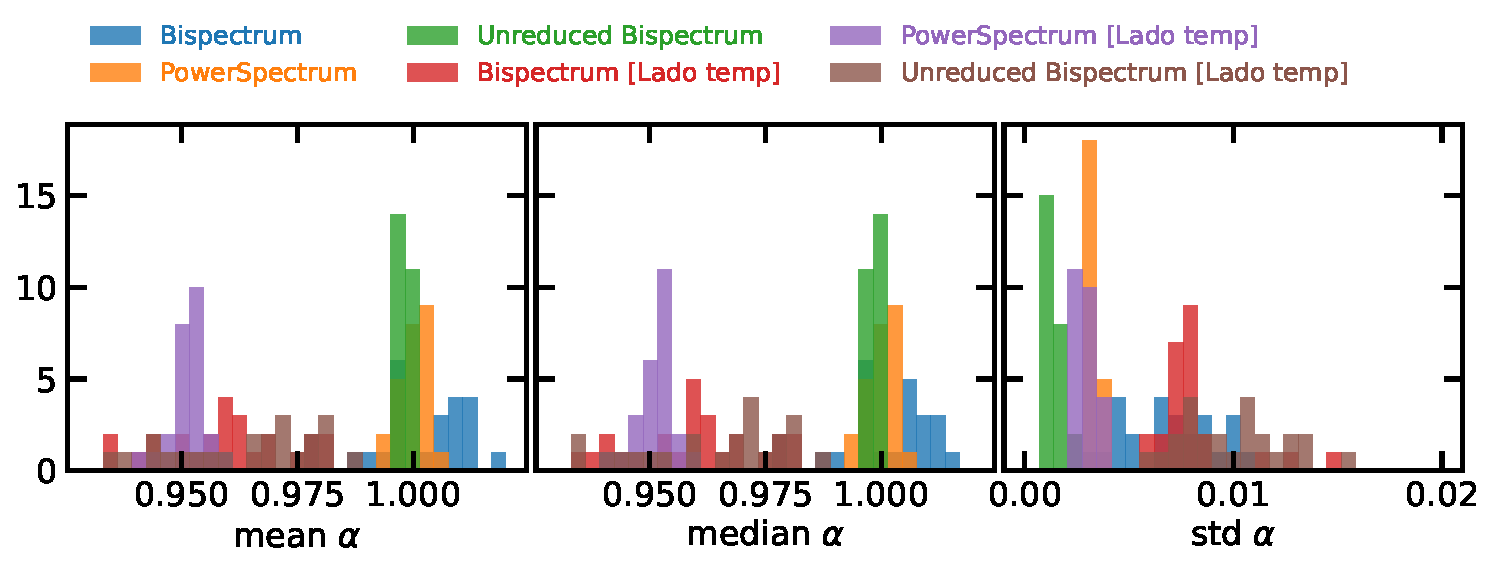
\includegraphics[width=\textwidth]{figures/constraints_ELGz1.pdf}
    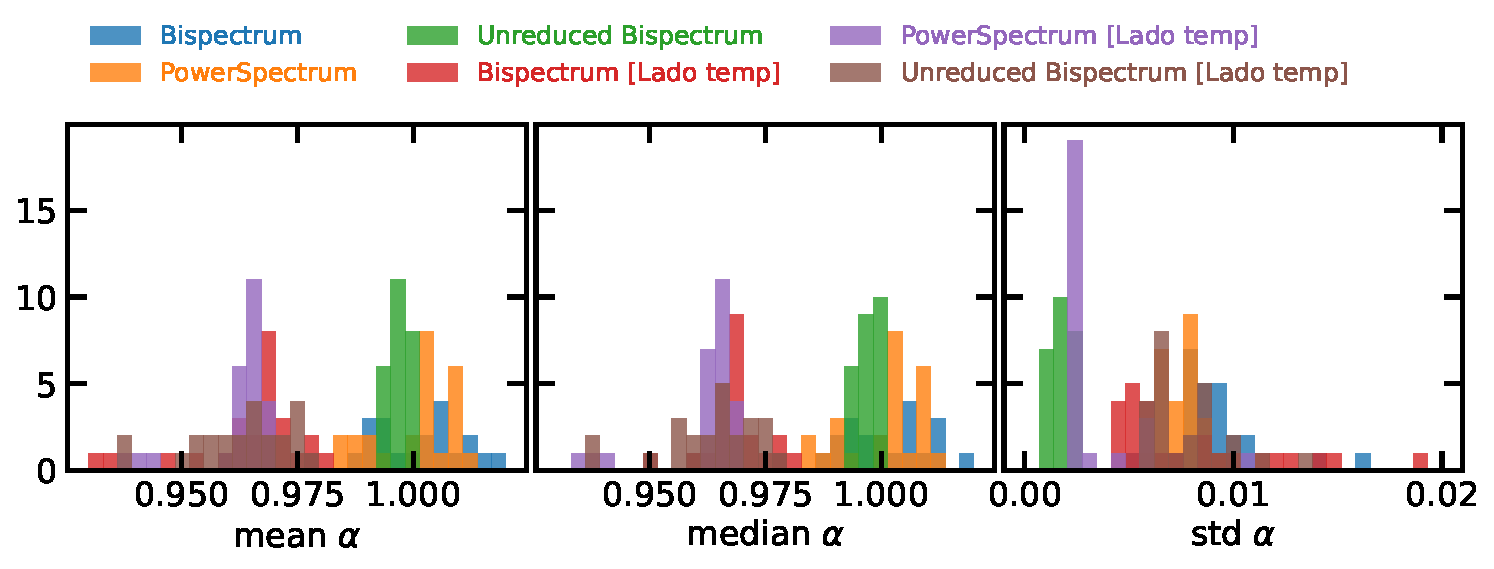
\includegraphics[width=\textwidth]{figures/constraints_QSOz2.pdf}    
    \caption{Mean, median, and standard deviation of BAO scale from 25 LRG (top), ELG (middle), and QSO (bottom) simulations.}
    \label{fig:constraints}
\end{figure*}


\begin{figure}
    \centering
    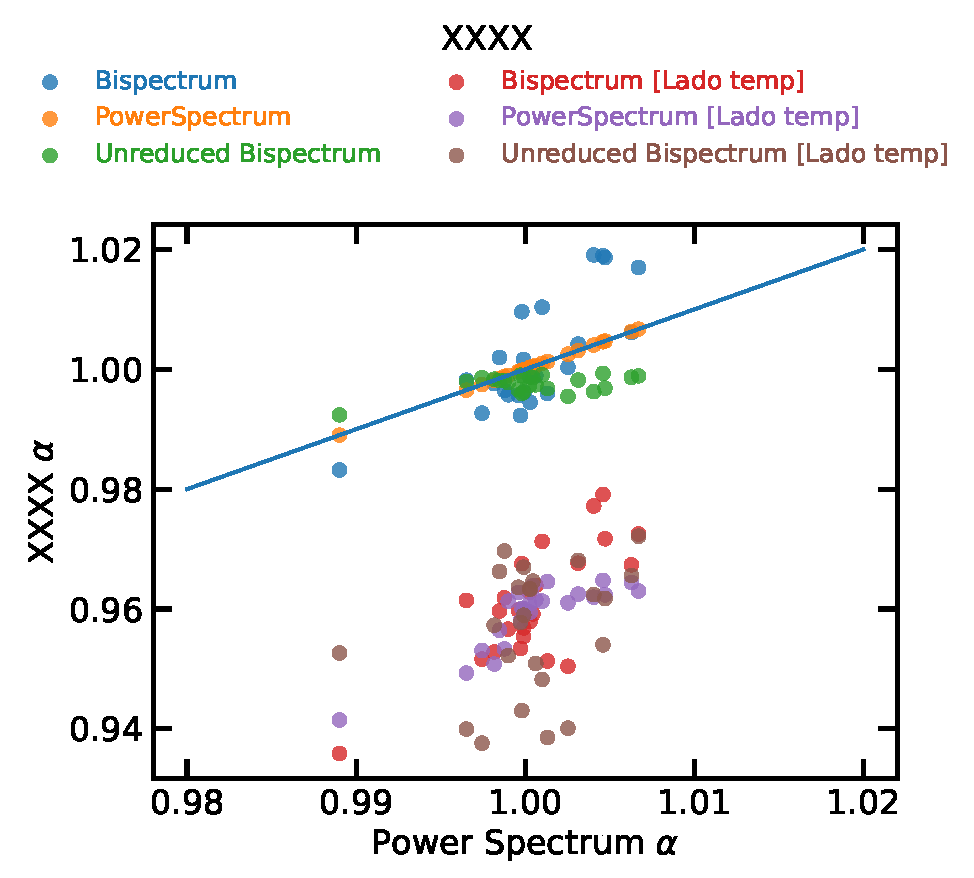
\includegraphics[width=0.45 \textwidth]{figures/constraints_scatter_LRGz0.pdf}
    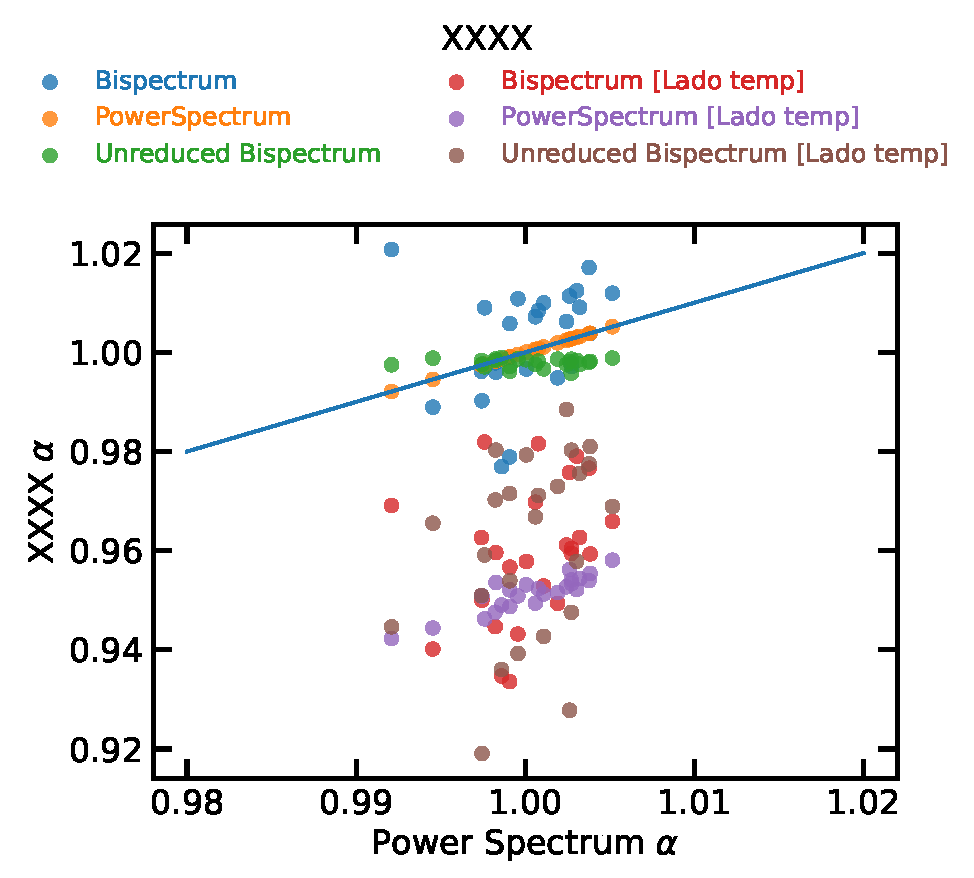
\includegraphics[width=0.45 \textwidth]{figures/constraints_scatter_ELGz1.pdf}
    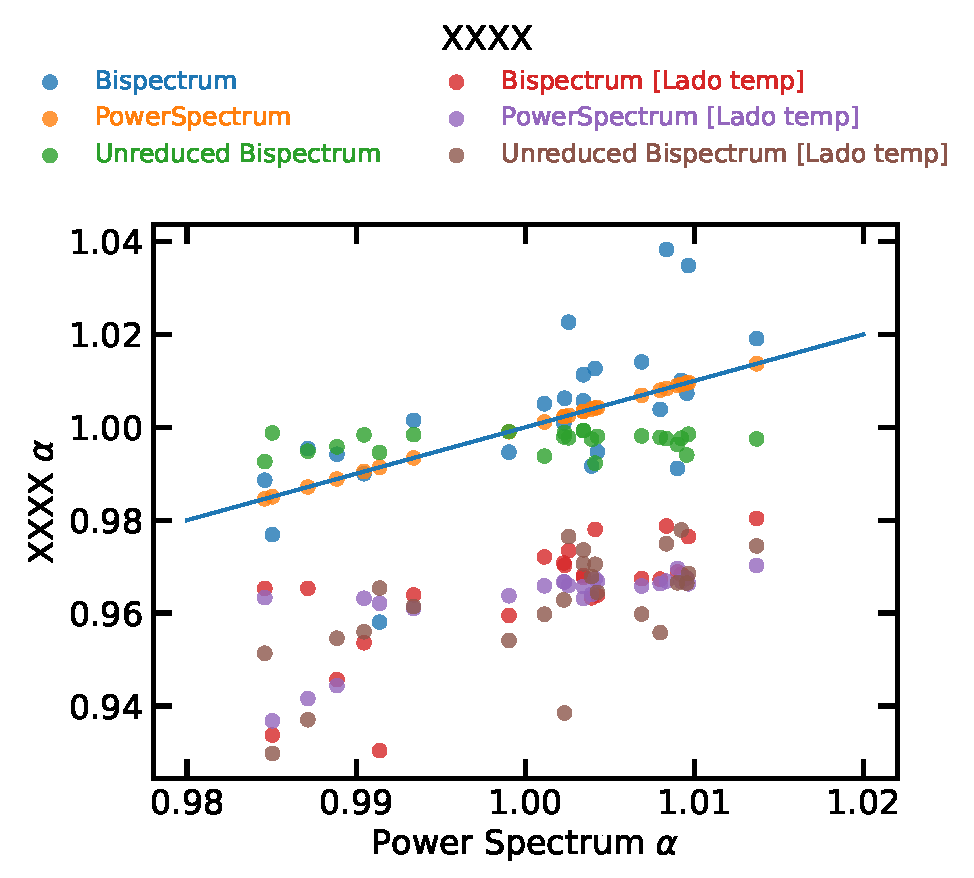
\includegraphics[width=0.45 \textwidth]{figures/constraints_scatter_QSOz2.pdf}
    \caption{BAO scale from various measurements vs that of power spectrum for 25 LRG (top), ELG (middle), and QSO (bottom) simulations.}
    \label{fig:scatter_cons}
\end{figure}
\section{Modeling the BAO}
\section{Covariances}
\label{sec:covariances}

We fit the BAO-only bispectra in \texttt{AbacusSummit} by minimizing the weighted squared difference between the measurements and the model, 
\begin{equation}
\label{eq:weightedsum}
    \chi^2(\alpha, \nu) = \Delta  \mathbf{B}^\mathrm{T} \mathbfss{W}\Delta \mathbf{B},
\end{equation}
where 
\begin{equation}
    \Delta  \mathbf{B}(\alpha, \nu) = \mathbf{B}_\mathrm{m} - \mathbf{B}_\mathrm{t}(\alpha, \nu),
\end{equation}
is the difference between measured and theoretical bispectra and $\mathbfss{W}$ is a positive definite weighting matrix that upweights the contribution of some linear combinations of $\Delta  \mathbf{B}$ to the $\chi^2$ compared to the others. The theoretical bispectrum depends on the BAO scale parameter $\alpha$ as well as nuisance parameters $\nu$. We expect the $\chi^2$ to achieve its minimum value at the true parameter $\alpha^\star$ as long as our model is unbiased and the average value of $\Delta  \mathbf{B}$ over many realizations is zero. The actual minimizer values $\widehat{\alpha}$ from individual realizations will be spread around the true value $\alpha^\star$ with some standard deviation $\sigma_\alpha^\star$. We will estimate $\sigma_\alpha^\star$ from the standard deviation of $\widehat{\alpha}$ values - $\widehat{\sigma}_\alpha$ - that we get from 25 \texttt{AbacusSummit} mocks. The fractional variance in our estimate of the error is expected to be
\begin{equation}
\label{eq:samplevariance}
    \frac{\mathrm{Std}(\widehat{\sigma}_\alpha)}{\sigma_\alpha^\star} = \sqrt{\frac{2}{N_\mathrm{sample}-1}}.
\end{equation}
$N_\mathrm{sample} = 25$ in our case which results in a 28 percent uncertainty. The \texttt{AbacusSummit} boxes cover 8 cubic Gigaparsecs of volume which is significantly larger than the BAO scale. We expect the errors on the $\widehat\alpha$ to scale as $V^{-1}$ for larger volumes. 

The main purpose behind the weighting matrix $\mathbfss{W}$ is to minimize $\sigma_\alpha^\star$ by upweighting bispectrum combinations that are measured more precisely compared to the noisy ones. The optimal weighting is achieved when 
\begin{equation}
    \label{eq:weightoptimal}
    \mathbfss{W} = \mathbfss{C}^{-1},
\end{equation}
 where $\mathbfss{C}^{-1}$ is the true inverse covariance of the bispectrum measurements. Another convenient property of the weights following Eq.~\eqref{eq:weightoptimal} is that when they are used the distribution of the $\alpha$ values in the Markov Chain Monte Carlo (MCMC) follows their true likelihood. This means that we can use the MCMC posterior distribution to estimate the error on our measurement of $\alpha$ which is more accurate than estimating it from a sample variance of a retrieved parameter from a small number of mocks, in which case the knowledge of the error on the measurement is limited by Eq.~\eqref{eq:samplevariance} \citep[see, e.g.,][for a comparison of two ways of estimating errors when combining BAO measurements.]{2022JCAP...05..040G}

Unfortunately, at this point in time, we do not have a large suite of high-fidelity simulations for estimating accurate inverse covariance of our bispectrum measurements. Instead, we try a few different options for the weighting matrix based on the theoretical expectation of how the bispectrum variance is expected to scale for Gaussian fields \citep{2017MNRAS.467..928G, 2019MNRAS.490.5931P, 2022PhRvD.106d3515H}. 

We try out three weighting schemes in our analysis
\begin{itemize}
\item Diagonal errors from \texttt{AbacusSummit} simulations
\item Correlated (non-diagonal) weighting from \texttt{Molino} simulations
\item And a theoretically computed weighting based on a simple Gaussian model with shot-noise
\end{itemize}

The diagonal errors are computed by simply looking at the variance of each bispectrum mode and ignoring cross-correlations. The resulting $\mathbfss{W}$ is diagonal which makes it numerically inexpensive to implement in our codes. Since this weighting scheme ignores cross-correlations between the modes and is based on a very small number of simulations, we don't expect it to be very optimal. We do expect it to provide us with a rough scaling between low and high wavenumber modes of the bispectrum. The fact that this weighting is derived from a significantly smaller number of mocks than the bispectrum modes that we use in our analysis is not a big problem for us since we are using Eq.~\eqref{eq:samplevariance} to estimate our errors. Even though we use MCMC to find $\widehat{\alpha}$ values, we do not try to interpret the width of the MCMC posterior as our posterior likelihood   and the usual problems associated with numerical inverse covariance matrices and Hartlap factors \citep{2007A&A...464..399H, 2013MNRAS.432.1928T, 2013PhRvD..88f3537D, 2014MNRAS.439.2531P} do not apply to our analysis. 

To get a sense of how the correlations between different bispectrum modes may affect the weighting we compute a reduced covariance matrix from 15,000 \texttt{Molino} simulations. The high number of simulations makes the coefficients of the reduced covariance matrix highly accurate. These cross-correlation coefficients give us some idea of how much the bispectrum modes measured from massive galaxies at lower redshifts can be correlated. We rescale this reduced covariance matrix by the standard diagonal errors described in the previous paragraph to get a weighting that accounts for the relative noise it different wavenumbers and the covariance between different wavenumbers at the same time. 

Finally, we estimate the inverse covariance matrix of bispectrum measurements theoretically based on the expectation from purely Gaussian fields and accounting for Poisson shot noise and use it as our weight. This estimate is going to be off at higher wavenumbers where the non-Gaussian effects will diverge from our computations, but we still expect this weighting to be close to optimal and get the correct relative weighting between small wavenumbers that are dominated by cosmic variance and large wavenumbers that are dominated by shot noise. 

\textcolor{red}{LS: once we have all results we will write a sentence here summarizing our findings. Which weightings resulted in a tighter distribution of $\tilde{\alpha}$.}
\section{BAO fits}
\label{sec:fits}

\textcolor{red}{one or two options for the model. nuisance parameters.}

\textcolor{red}{Glam template. Linear template.}

\textcolor{red}{spread of measured alpha over 25 FirstGens}

\textcolor{red}{alongside with alpha fits to the power spectrum}

\textcolor{red}{experiment with some choices.}

\textcolor{red}{sigma alpha from the posterior (as a function of k)}

\textcolor{red}{min $\chi^{2}$ vs alpha for P(k), B(k1, k2, k3), P+B BAO and BAOless templates. Look into the scatter in the detection significance across the realizations.}

% \begin{figure*}
% 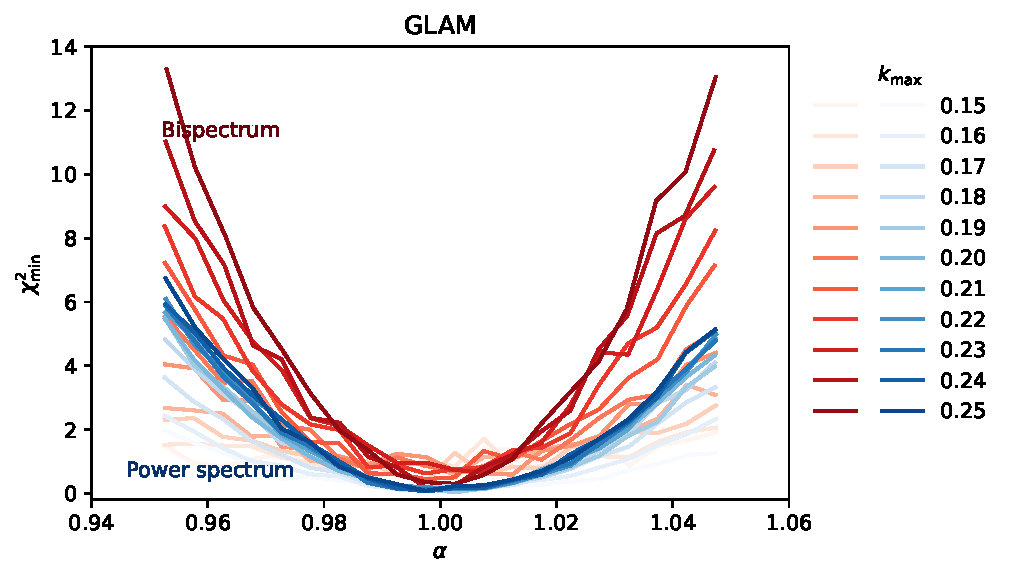
\includegraphics[width=0.48\textwidth]{chi2_GLAM.pdf}
% 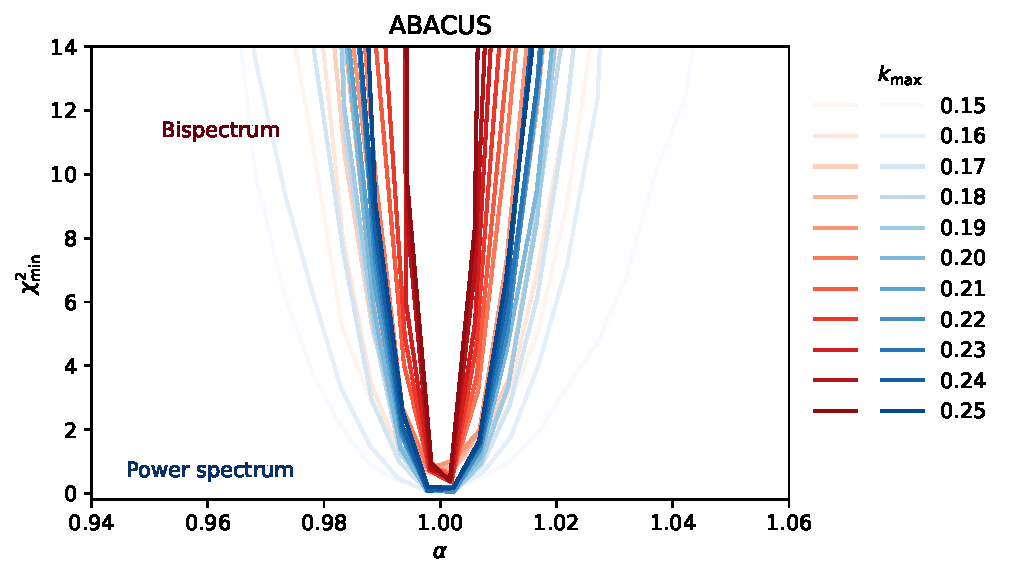
\includegraphics[width=0.48\textwidth]{chi2_ABACUS.pdf}
% 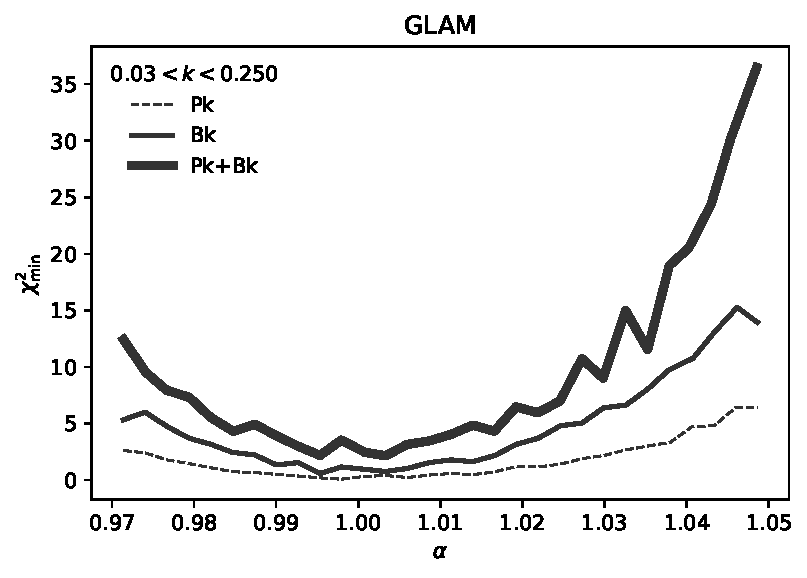
\includegraphics[width=0.48\textwidth]{chi2alpha_glam.pdf}
% 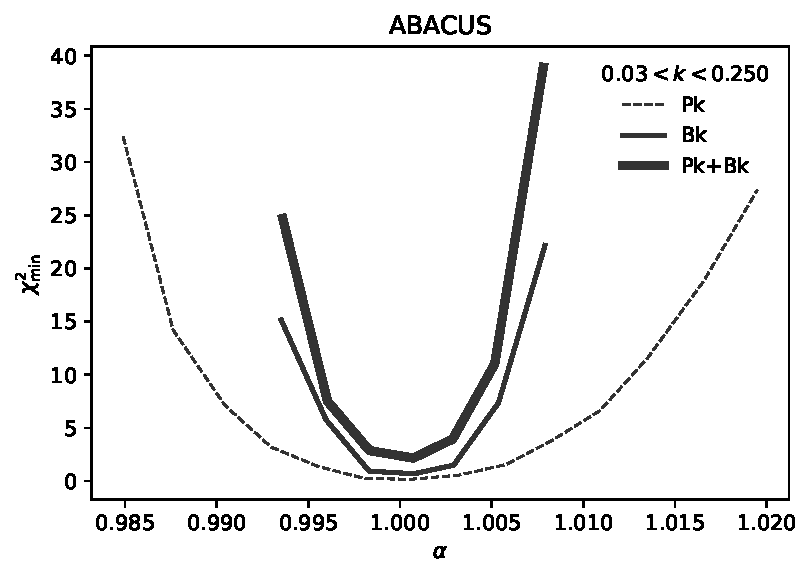
\includegraphics[width=0.48\textwidth]{chi2alpha_abacus.pdf}
% \caption{Marginalized minimum $\chi^{2}$ as a function of the BAO peak $\alpha$}\label{fig:chi2alpha}
% \end{figure*}

% \begin{figure*}
% 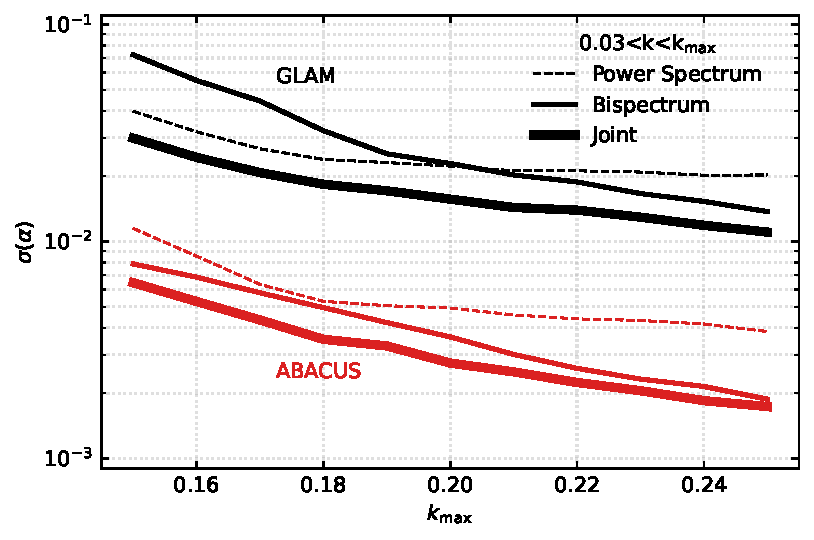
\includegraphics[width=0.9\textwidth]{sigma_kmax.pdf}
% \caption{Dispersion in the BAO peak $\alpha$ as a function of the maximum wavenumber $k_{\rm max}$}
% \end{figure*}
\section{Conclusion}\label{sec:conclusion}
Where you provide the take-home message.
%\section*{Acknowledgements}
Thank anonymous referee, sponsors, your colleagues. 
%\section*{Data Availability}
\label{sec:dataavail}

Instruct how data used in this work can be accessed.

% references
\bibliographystyle{mnras}
\bibliography{refs} 
\appendix
\section{Templates}\label{sec:templates}
The templates for power spectrum and bispectrum are validated in \cite{behera2013}, and we briefly summarize the methods. These templates are used to qualitatively assess the location and magnitude of baryonic oscillations in power spectrum and bispectrum.

\subsection{Power spectrum}
The fitting function or template for the power spectrum is given in \citep{1998ApJ...496..605E}, which assumes a general cold dark matter-baryon cosmology and corrects for the suppression of clustering on small scales, e.g., below the sound horizon. The power spectrum can be described as the multiplication of the primordial power spectrum and the square of the transfer function, which for a zero baryon cosmology is given by,
\begin{equation}
    T_{0} = \frac{\ln(2e+1.8q)}{\ln(2e+1.8q) + C_{0} q^{2}}
\end{equation}
where,
\begin{align}
    C_{0} &= 14.2 + \frac{731}{1 + 62.5q}\\
    q &= (\frac{k}{h{\rm Mpc}^{-1}})\frac{\Theta^{2}_{\rm CMB}}{\Omega_{0}h}
\end{align}
where $\Theta$ is the temperature of the cosmic microwave background and $\Omega_{0}$ is the total matter density. The damping on large scales due to baryons is described by,
\begin{equation}
    \Gamma(k) = \Omega_{0}h[\alpha_{\Gamma} + \frac{1-\alpha_{\Gamma}}{1 + (0.43ks)^{4}}] 
\end{equation}
where
\begin{align}
    \alpha_{\Gamma} &=1-0.328\ln(431\Omega_{0}h^{2})\frac{\Omega_{b}}{\Omega_{0}}\nonumber\\
    &+ 0.38\ln(22.3\Omega_{0}h^{2}) (\frac{\Omega_{b}}{\Omega_{0}})^{2}
\end{align}
where $\Omega_{b}$ represents the baryon density today. 


\subsection{Bispectrum}
Scoccimarro, Couchman, and Frieman (1998): bispectrum template with plane-parallel approx and damping factor (for nonlinear effects due to velocity dispersion).



% % % Don't change these lines
\bsp	% typesetting comment
\label{lastpage}
\end{document}